% task2.tex — Shallow Anomaly Detection with One-Class SVM

\section{SHALLOW ANOMALY DETECTION} \label{sec:task2}

In this section, we investigate One-Class Support Vector Machine (OC-SVM) for anomaly detection under three training configurations: normal data only (novelty detection), all data (outlier detection), and mixed data with varying anomaly contamination ratios.

% --- OC-SVM Normal Only ---
\subsection{OC-SVM with Normal Data Only (Novelty Detection)} \label{sec:ocsvm_normal}

    In novelty detection, the OC-SVM is trained exclusively on normal traffic, learning a tight boundary around the normal data manifold.
    The key hyperparameter is $\nu$, which controls the upper bound on the fraction of training errors.
    Since the training data is purely normal, $\nu$ should reflect the expected fraction of noisy or edge-case normal samples.
    We evaluated four values: $\nu \in \{0.001, 0.01, 0.05, 0.5 \text{ (default value)}\}$.

    \begin{table}[H]
        \centering
        \begin{tabular}{@{}lcc@{}}
            \toprule
            \textbf{$\nu$} & \textbf{Train F1-Macro} & \textbf{Test F1-Macro} \\
            \midrule
            0.001             & 0.9058 & 0.7382 \\
            0.01              & 0.9039 & 0.7401 \\
            \textbf{0.05}     & \textbf{0.9026} & \textbf{0.7477} \\
            0.5 (default)     & 0.6378 & 0.4647 \\
            \bottomrule
        \end{tabular}
        \caption{OC-SVM (Normal-Only): impact of $\nu$ on performance.}
        \label{tab:nu_comparison}
    \end{table}

    \noindent
    We selected $\nu = 0.05$ as the optimal value, as it achieves the highest test F1-Macro (0.7477), allowing the model to exclude approximately 5\% of normal samples as edge-case noise and creating a slightly looser boundary that generalizes better.
    However, the variation in performance among the three lower values tested ($\nu \in \{0.001, 0.01, 0.05\}$) is minimal. 
    This highlights that the $\nu$ parameter is not a strict limit, but rather an upper boundary to the number of anomalies the model expects. 
    The default value $\nu = 0.5$ forces instead 50\% of normal training samples to lie outside the decision boundary, systematically undermining the normality model and collapsing test F1-Macro to 0.4647.

% --- OC-SVM All Data ---
\subsection{OC-SVM with All Data (Outlier Detection)} \label{sec:ocsvm_all}

    When training on the full dataset (normal + anomalies), the OC-SVM operates as an \emph{outlier detector}.
    We set $\nu$ to the true contamination rate: $\nu = 4305/15063 \approx 0.286$.
    The Normal-Only model outperforms the All-Data model by approximately \textbf{10 percentage points} in test F1-Macro (0.7477 vs.\ 0.6484), demonstrating that novelty detection yields a more effective decision boundary than outlier detection on contaminated data.

% --- Sensitivity Analysis ---
\subsection{Sensitivity Analysis: Impact of Anomaly Contamination} \label{sec:sensitivity}

    To quantify the effect of training data contamination, we trained OC-SVMs with increasing proportions of anomalous data (0\%, 10\%, 20\%, 50\%, 100\%), setting $\nu$ proportionally to the anomaly ratio at each level.

    \begin{figure}[H]
        \centering
        \begin{minipage}{0.47\linewidth}
            \centering
            \makeatletter\def\@captype{table}\makeatother
            \resizebox{\linewidth}{!}{%
                \begin{tabular}{@{}rccc@{}}
                    \toprule
                    \textbf{Anomaly \%} & \textbf{$\nu$} & \textbf{Train F1-Macro} & \textbf{Test F1-Macro} \\
                    \midrule
                    \textbf{0\%} (Normal-Only)  & 0.01  & \textbf{0.9039} & \textbf{0.7401} \\
                    10\%                         & 0.038 & 0.6628 & 0.5137 \\
                    20\%                         & 0.074 & 0.6779 & 0.5589 \\
                    50\%                         & 0.167 & 0.7226 & 0.5975 \\
                    100\% (All-Data)             & 0.286 & 0.7364 & 0.6482 \\
                    \bottomrule
                \end{tabular}%
            }
            \caption{Sensitivity analysis: impact of anomaly\\ contamination on OC-SVM performance.}
            \label{tab:sensitivity}
        \end{minipage}\hfill
        \begin{minipage}{0.50\linewidth}
            \centering
            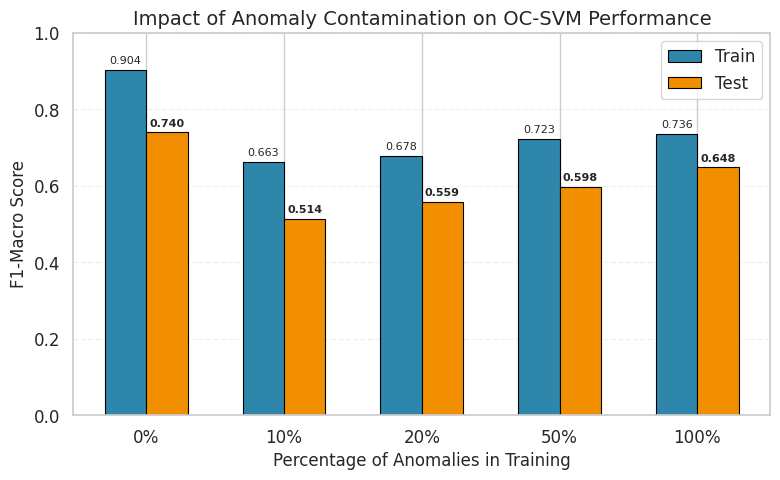
\includegraphics[width=\linewidth]{images/task2/task2_sensitivity_analysis_combined.png}
            \caption{F1-Macro scores across anomaly contamination levels.}
            \label{fig:task2_sensitivity}
        \end{minipage}
    \end{figure}

    \vspace{-0.2cm}

    \noindent
    The results exhibit a \textbf{non-monotonic relationship} between contamination level and test F1-Macro: performance degrades sharply at 10\% contamination (F1 = 0.514) before partially recovering as contamination reaches 100\% (F1 = 0.648).
    This recovery reflects $\nu$ growing large enough to absorb the anomaly fraction, though no contaminated configuration approaches the clean baseline (F1 = 0.740).
    Small contamination levels are the most damaging because the model receives conflicting signals about what constitutes normal behavior, yet $\nu$ remains too small to properly account for the anomalies present.

% --- Robustness ---
\subsection{Robustness Evaluation} \label{sec:robustness}

    We compared three representative models on the test set to assess generalization and per-attack detection robustness.

    \vspace{-0.2cm}

    \begin{table}[H]
        \centering
        \begin{tabular}{@{}lccc@{}}
            \toprule
            \textbf{Model} & \textbf{Train F1} & \textbf{Test F1} & \textbf{Most Missed (FNR\%)} \\
            \midrule
            Normal-Only ($\nu{ = }0.05$) & 0.9026 & \textbf{0.7477} & DoS (23.6\%) \\
            All-Data ($\nu{ = }0.286$)   & 0.7364 & 0.6484          & DoS (41.7\%) \\
            10\% Anomalies               & 0.6628 & 0.5137          & DoS (77.2\%) \\
            \bottomrule
        \end{tabular}
        \vspace{0.5em}
        \caption{Robustness evaluation on test set, including Train F1 and per-attack False Negative Rate (FNR).}
        \label{tab:robustness}
    \end{table}   
    
    \vspace{-0.5cm}
    
    \noindent
    The Normal-Only model ($\nu = 0.05$) achieves the best performance on both the training and test set ( \Cref{tab:robustness}). 
    This confirms that the model generalizes pretty well and does not overfit to specific training anomalies, while the other two models, trained on contaminated data, show a significant performance drop.

    On the test set, errors are split between False Positives (normal traffic flagged as anomalous due to tight boundaries) and False Negatives (missed anomalies).
    Per-attack analysis on the Normal-Only model ($\nu = 0.05$) reveals that DoS attacks are the hardest to detect, with 609 of 2,577 samples misclassified (FNR = 23.6\%).
    This evasion occurs because DoS patterns (especially low-rate attacks) closely mimic legitimate high-traffic scenarios.
    Conversely, Probe attacks are highly identifiable, achieving an FNR of 2.8\% (31 of 1,097 samples missed) since scanning and reconnaissance activities diverge clearly from normal network patterns.

    Training contamination is particularly damaging for DoS detection: the FNR rises to 41.7\% in the All-Data model and peaks at 77.2\% with 10\% contamination.
    This represents a \textbf{3.3$\times$ increase in missed DoS attacks} from minimal training pollution, highlighting how conflicting signals degrade decision boundaries.
    While the subtle signatures of R2L attacks make them theoretically the most challenging class to detect, their complete absence from the test set prevents any empirical evaluation of their robustness.
    Nevertheless, on the evaluated classes, the Normal-Only approach achieves the best precision-recall balance, confirming that novelty detection is the most robust strategy when clean data is available.
